% document formatting
\documentclass[10pt]{article}
\usepackage[utf8]{inputenc}
\usepackage[left=1in,right=1in,top=1in,bottom=1in]{geometry}
\usepackage[T1]{fontenc}
\usepackage{xcolor}

% math symbols, etc.
\usepackage{amsmath, amsfonts, amssymb, amsthm}

% lists
\usepackage{enumerate}

% images
\usepackage{graphicx} % for images

% code blocks
\usepackage{minted, listings} 

% verbatim greek
\usepackage{alphabeta}

\graphicspath{{./assets/images}}

\newcommand{\solution}{\textbf{Solution:}} 
\newcommand{\example}{\textbf{Example: }}
\newcommand{\R}{\mathbb{R}}

\title{BIOMATH 208 Week 5}

\author{Aidan Jan}
\date{\today}

\begin{document}
\maketitle
\subsection*{Review}
A manifold:
\begin{enumerate}
    \item $\mathcal{M}$ a set (often a subset of a bigger space, like a donut)
    \item A topology (open sets, sets that don't include boundary continuous functions)
    \item An atlas which is a set of charts.
    \begin{itemize}
        \item Each chart: $u \subseteq \mathcal{M}$ (coordinate neighborhood)
        \item $x \::\: u \rightarrow \R^d$ (coordinate map)
        \item $x$ must be continuous and invertible and have continuous inverse
        \item "locally" find a subset $u$, can be small $\rightarrow$ "looks like $\R^d$"
    \end{itemize}
    \item Every point on the manifold needs to be in at least one coordinate neighborhood
\end{enumerate}
\begin{center}
    \includegraphics*[scale=0.9]{W5_5.png}
\end{center}
Compatibility:
\begin{itemize}
    \item Smoothness compatibility: If all chart transition maps are continuously differentiable, the atlas is smoothness compatible, and we have a smooth manifold.
    \item Want smooth manifolds so we can do optimization
    \begin{itemize}
        \item E.g., if $\mathcal{M} = (-1, 1)$ and our charts are $x(p) = p$ and $y(p) = p^3$, this does not work because $y(p)$ is not differentiable at the origin.
    \end{itemize}
\end{itemize}

\section*{Groups}
\subsection*{Motivation}
A common data type in imaging which is not vector valued, are sets called groups.
\begin{itemize}
    \item Typically groups are used to describe transformations, such as those that can be used to align multiple modalities of imaging data.
    \item When the family of transformations we consider also forms a smooth manifold, this is called a Lie (Pronounced: Lee) group.
\end{itemize}
\subsection*{Definition}
A set $G$, together with a binary operations $\circ \::\: G \times G$ is called a group if it satisfies the following properties.  Here, let $f, g, h \in G$:
\begin{itemize}
    \item Associativity: $(f \circ g) \circ h = f \circ (g \circ h) = f \circ g \circ h$
    \item Neutral Element: "Identity Element", $i \in G$, such that $f \circ i = i \circ f = f$
    \item Inverse Element: There exists a "$f^{-1}$", such that $f^{-1} \circ f = f \circ f^{-1} = i$
\end{itemize}
This is very similar to vector spaces with $+$, but there is no C (commutativity).  The $\circ$ operation used here is composition.\\\\
An example of a group is matrix multiplication, because C is missing.
\begin{itemize}
    \item When multiplying matrices, order matters.  Therefore, it is not commutative.
\end{itemize}
\subsection*{Other Properties}
\subsubsection*{Uniqueness of Identity}
There is only one identity.  Suppose that $a$ and $b$ are both identity elements, but are distinct.  Then,
\begin{align*}
    a \circ b &= b \hspace{1.5cm} \text{because a is identity}\\
    a \circ a &= a \hspace{1.5cm} \text{because b is identity}\\
    \intertext{Therefore, by the transistivity of the equals sign,}
    a &= b
\end{align*}
Therefore, $a = b$, which contradicts our assumption that there are two distinct identities.
\subsubsection*{Uniqueness of Inverse}
There is only one inverse.  Suppose that $a$ has two distinct inverses, $b$ and $c$.  Then,
\begin{align*}
    c \circ a \circ b &= (c \circ a) \circ b\\
    &= c \circ (a \circ b)\\
    \intertext{Since c is an inverse of a, we get}
    &= i \circ b
    \intertext{However, since b is an inverse of a, we get}
    &= i \circeq
\end{align*}
Therefore, $b = c$, which contradicts our assumption that there are two distinct inverses.
\subsubsection*{Example: Rotations in 2D}
\[\begin{pmatrix}
    \cos \theta & -\sin \theta \\ \sin \theta & \cos \theta
\end{pmatrix}\]
In this case, $\theta$ and $\theta + 2\pi$ give the same rotations!  However, in terms of groups, they are considered to be the same, since a cosine or sine of adding 2$\pi$ can be simplified.

\subsection*{Cayley Tables}
Rotations about arbitrary angles are infinite groups.\\\\
Definition:
\begin{itemize}
    \item For finite groups, we can list the result of binary operations in a table.  The first input to $\circ$ will be the row, the second input to $\circ$ will be the column, and the result will be in the corresponding cell.
    \begin{center}
        \includegraphics*[scale=0.8]{W5_1.png}    
    \end{center}
    \item Complete representation!  Everything you might want to know about the group.
\end{itemize}

\subsubsection*{Example: One element group}
The simplest group has only one element.  $G = \{a\}$ (the set)
\begin{center}
    \begin{tabular}{c|c}
        $\circ$ & $a$ \\ \hline
        $a$ & $a \circ a = a$
    \end{tabular}
\end{center}
\begin{itemize}
    \item $a$ is identity.
    \item $a = a^{-1}$
\end{itemize}

\subsubsection*{Example: Two element group}
We can build a two element group, for example, modeling reflections
\begin{center}
    \begin{tabular}{c|cc}
        $\circ$ & $a$ & $b$ \\ \hline
        $a$ & $a$ & $a \circ b = b$ \\
        $b$ & $b \circ a = b$ & $b \circ b = a$
    \end{tabular}
\end{center}
We could think of $G = \{1, -1\}$ and $\circ = \cdot$.
\begin{itemize}
    \item For the bottom right corner, $b$ must have an inverse, and it cannot be $a$, therefore it must be $b$.
    \item The same table can represent more than one set and more than one operator.
\end{itemize}

\subsubsection*{Example: Three element group}
We can build a 3 element group, for example, rotations by 120 degrees.
\begin{center}
    \begin{tabular}{c|ccc}
        $\circ$ & 0 & 120 & 240 \\ \hline
        0 & 0 & 120 & 240 \\
        120 & 120 & 240 & 0 \\
        240 & 240 & 0 & 120
        \end{tabular}
\end{center}
We could think of these elements as numbers, and $\circ$ as addition mod 360.\\\\
Or\dots we could think of 0 as $\begin{pmatrix}1 & 0 \\ 0 & 1\end{pmatrix}$, 120 as $\begin{pmatrix}-0.5 & -0.870 \\ 0.870 & -0.5\end{pmatrix}$, etc., and $\circ$ as matrix multiplication.

\subsubsection*{Example: Integers with Plus}
\begin{center}
    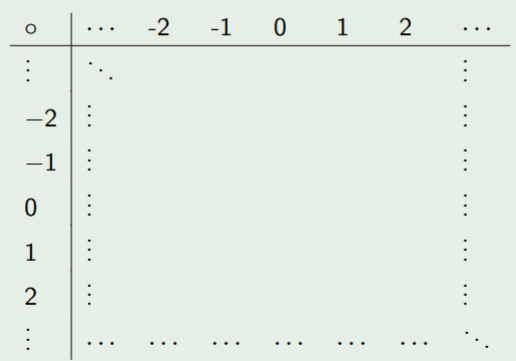
\includegraphics[scale=0.9]{W5_2.png}
\end{center}
Every sum of integer is also an integer.  In this case, integers are an infinite group since it is closed if $\circ = +$.  Additionally,
\begin{itemize}
    \item The neutral element of the integer set is 0
    \item The inverse any integer $a$ is $-a$.
\end{itemize}

\subsubsection*{Example: Permutations}
Permutations refer to how we can rearrange the elements.
\begin{center}
    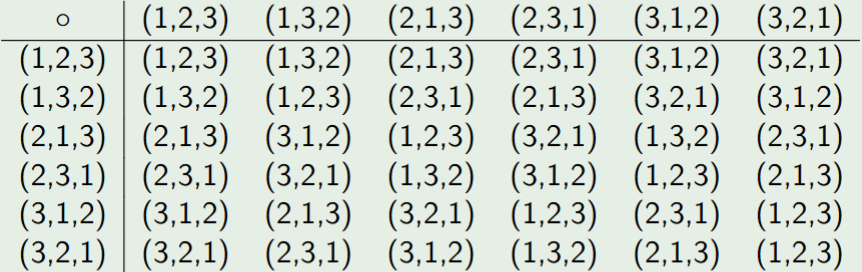
\includegraphics[scale=0.8]{W5_3.png}
\end{center}
These can also be represented as elementary matrices acting by matrix multiplication.  The objects that get transformed are related to the objects doing the transforming.

\subsection*{Group Actions}
Groups often represent transformations, and they therefore act on the objects they transform.
\subsubsection*{Left Group Action}
Let $\mathcal{I}$ be some set of objects we act on, then $\cdot \::\: G \times \mathcal{I} \rightarrow \mathcal{I}$ is called a left group action if it respects group properties.  With $I \in \mathcal{I}$, $f, g \in G$, $i$ = identity $\in G$, we require:
\begin{enumerate}
    \item Identity: $i \cdot I = I$
    \item Compatibility: $ g \cdot (f \cdot I) = (g \circ f) \cdot I$
    \begin{itemize}
        \item LHS of equation: We act on the image twice
        \item RHS of equation: We compose the actions and act on the image once.
    \end{itemize}
\end{enumerate}

\subsubsection*{Right Group Action}
Let $\mathcal{I}$ be some set of objects we act on, then $\cdot \::\: \mathcal{I} \times G \rightarrow \mathcal{I}$ is called a right group action if it respects group properties.  With $I \in \mathcal{I}$, $f, g \in G$, $i$ = identity $\in G$, we require:
\begin{enumerate}
    \item Identity: $I \cdot i = I$
    \item Compatibility: $ (I \cdot f) \cdot g = I \cdot (f \circ g)$
\end{enumerate}
Left and right group actions are the same if the operation is commutative.
\begin{itemize}
    \item This is like multiplication of matrices with vectors (e.g., on the right side), while left group action is like a covector multiplied by a matrix (e.g., on the left side).
\end{itemize}

\subsection*{Permutation and Reflection of Axes}
\begin{itemize}
    \item Discrete images are arrays indexed with three numbers: \texttt{I[i, j, k]}.
    \item Typically, we use a symbol like "RAS" to mean:
    \begin{itemize}
        \item The first axis points from left to right.
        \item The second axis points from posterior to anterior.
        \item The third axis points from inferior to superior.
    \end{itemize}
    \item The permutation group can act on an image (left action) to reorient it: RAS, RSA, ARS, ASR, SRA, SAR.
    \item Permutations and reflections can generate 48 combinations: (R/L, A/P, S/I).
\end{itemize}

\subsection*{Lie Group}
A Lie (pronounced like "lee") group is a group which is also a smooth manifold, which is compatible with its smooth structure.\\\\
Compatible means composition and inverse are differentiable functions of the coordinates.

\subsubsection*{Example: Addition of Reals}
The real numbers with addition is a Lie group.  We know the real numbers form a manifold, so first we can check this is a group:
\begin{itemize}
    \item Associtivity: $(a + b) + c = a + (b + c)$   (and closed under the group operation, e.g., $G \times G \rightarrow G$)
    \item Neutral element: $0$
    \item Inverse element: $a^{-1} = -a$ 
\end{itemize}
Then, we check that its group structure is compatible:  We will pick the natural chart to make this easy, e.g., $x(p) = p$, just use the real number
\begin{itemize}
    \item $\circ$: $\circ (x, y) = x + y$, $\partial_0 \circ(x, y) = 1$, $\partial_1 \circ(x, y) = 1$ 
    \begin{itemize}
        \item These need to be differentiable functions in this chart and in any chart in our smoothly compatible atlas. (which they are)
    \end{itemize}
    \item $^{-1}$: $^{-1}(x) = -x$
\end{itemize}

\subsubsection*{Example: Multiplication of Positive Reals}
The positive real numbers with multiplication is a Lie group.  We know the positive real numbers form a manufold, so first we can check this is a group:
\begin{itemize}
    \item Associativity: $(a \cdot b) \cdot c = a \cdot (b \cdot c)$  (This does meet the closure ($G \times G \rightarrow G$) requirement, since multiplying two positive numbers will yield a positive number.)
    \item Neutral element: $1$
    \item Inverse element: $a^{-1} \cdot \frac{1}{a} \in \R^+$
\end{itemize}
Then we check that its group structure is compatible:
\begin{itemize}
    \item $\circ$:$\circ(x, y) = xy$, $\partial_0 \circ(x, y) = y$, $\partial_1 \circ(x, y) = x$
    \item $^{-1}$: $^{-1}(x) = \frac{1}{x}$, $\partial_0^{-1} (x) = -\frac{1}{x^2}$, which is well defined as long as $x \neq 0$.
\end{itemize}

\subsubsection*{Aside: Is addition of positive reals a lie group?}
$\R^+$ with $+$ (instead of multiplication) is NOT a Lie group, because there is no identity, neither is there an inverse.

\subsection*{Group Homomorphisms}
Let $f$ be a function mapping elements of a group $G$, to elements of a group $H$.  It is called a group homomorphism if it is compatible with the laws of compositions.  If $a, b \in G$, we require:
\[f(a \circ_G b) = f(a) \circ_H f(b)\]
Left side: composition in the group $G$.  Right side: composition in the group $H$.
When we introduced linear maps, we said that it is a function compatible with $+$ and $\cdot$.

\subsubsection*{Example: The Exponential Map}
The exponential function maps $(\R, +) \rightarrow (\R^{+}, \cdot)$.  For $a, b \in \R$, we have
\[\exp(a + b) = \exp(a) \cdot \exp(b)\]
It will be very useful to work with maps like these from a vector space (where it is easy to do computations) to a group (which models our data).

\subsubsection*{Example: Square Matrices}
Square matrices are not a Lie group.\\\\
This is because square matrices have no inverse!  E.g., the 0 matrix doesn't have an inverse.  (All the matrices form a group with $+$).

\subsubsection*{Example: General Linear Groups}
The invertible $n \times n$ matrices do form a Lie group with matrix multiplication.\\\\
To prove:
\begin{enumerate}
    \item This is a smooth manifold
    \item Show that it is a group
    \item Show that matrix multiplication and inverse are differentiable in some chart.
\end{enumerate}
First, we want to show that this is a smooth manifold.  In this case, $\R^{n \times n}$ is a smooth manifold.  What happens when we remove matrices that are not invertible?\\\\
To do this, we introduce $f \::\: \R^{n \times n} \rightarrow \R$, and $f(A) - \text{det}(A) \rightarrow 0$ if and only if $A$ is not invertible.
\[\mathcal{M} = f^{-1}(\R \backslash \{0\})\]
$f$ is continuous (polynomial).  $\R \backslash \{0\}$ is an open set, and since the inverse of an open set is an open set, $\mathcal{M}$ is also an open set.  To define an atlas for the sqwuare matrices, just intersect coordinate neighborhoods with this $n$.  This produces a smooth manifold of dimension $n^2$.\\\\
Next, we want to show that this is a group.  In this case, we define:
\begin{itemize}
    \item $\circ$: matrix multiplication
    \item neutral element: identity matrix
    \item inverse element: $A^{-1}$  (by construction we know it exists)
\end{itemize}
Finally, we want to show that matrix multiplication and inverse are differentiable in some chart.  $\circ$ and $A^{-1}$ are smooth functions of parameters, so we can use the "natural" chart.  (write down the $n^2$ numbers in an array)\\\\
Therefore, $AB$ (matrix multiplcation) is a quadratic function of the matrix entries, which is differentiable.\\\\
Additionally, $A^{-1}$ is a rational function (ratio of polynomials) of the matrix entries.\\\\
Therefore, this is a matrix Lie group!

\subsubsection*{Example: Affine Transformations}
Affine transformations consist of a linear transformation and a translation.  They can be represented by matrix multiplication in homogeneous coordinates.  (Also mentioned in graphics classes, homogeneous coordinates is when you take the vector to be transformed, and add a 1 at the bottom.  You would add a 0 at the bottom of points.)
\begin{align*}
    \begin{pmatrix} L & T \\ 0 & 1 \end{pmatrix} \begin{pmatrix} v \\ 1 \end{pmatrix} &= \begin{pmatrix} Lv + T \\ 1 \end{pmatrix}
\end{align*}
\begin{itemize}
    \item In the above example, $T$ is a vector, and $L$ is a square matrix.  $v$ is the vector to be transformed.
    \item The $0$ added below the $L$ is a zero row vector. 
    \item In this case, judging by the end product, we applied a translation.  The vector $v$ has been translated by vector $T$ (after being transformed by $v$).
    \item Note that this transformation is \textit{not linear} in terms of $v$, but it \textit{is linear} in terms of $\begin{pmatrix} v \\ 1 \end{pmatrix}$.
    \item The result is also a Lie group, just like the input.
\end{itemize}

\subsubsection*{Example: Translations}
Restricting $L = I$ (identity matrix) gives the translation group, with matrix multiplication as the binary operation.  Translation group could also be modeled as vectors with addition.
\[\begin{pmatrix} I & T \\ 0 & 1 \end{pmatrix} \begin{pmatrix} v \\ 1 \end{pmatrix} = \begin{pmatrix} v + T \\ 1 \end{pmatrix}\]
$+$ can also be written as a matrix group with matrix multiplication as the composition law.
\begin{itemize}
    \item Recall that $+$ is normally not a linear map.
\end{itemize}
It turns out that every Lie group, with finite dimension, can be expressed as matrix multiplication.

\subsection*{Example: Sizes}
Images can be transformed by scaling (e.g., magnification factors), and imaging data can represent scales (e.g., multiples of some standard size).
\begin{center}
    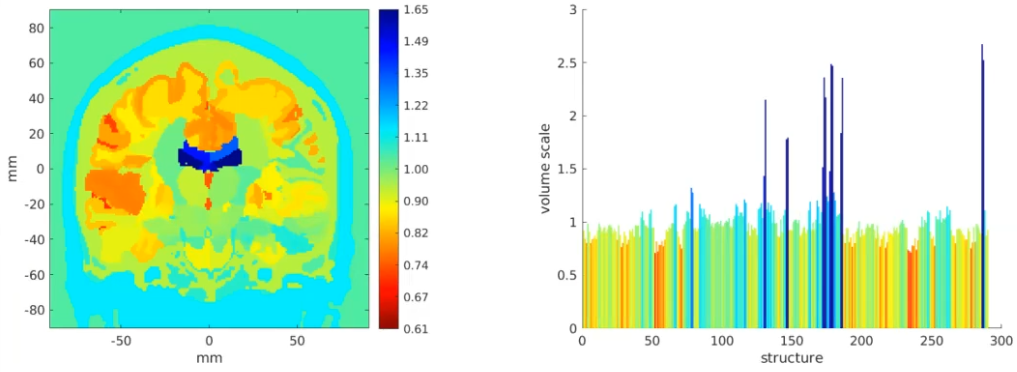
\includegraphics[width=\textwidth]{W5_4.png}
\end{center}
The above image shows 287 structures in the brain, and the color shows how different that part of the brain is compared to the average person's brain, in terms of size.  (1.00 means it is the same as a normal brain.)
\begin{itemize}
    \item Notice that there are no negative numbers.  (0 means the structure is not present)
\end{itemize}

\subsubsection*{Example: Charts for Sizes}
In extrinsic coordinates, we can write these transforms as $sI$, for $x \in \R^+$ and $I$ the identity matrix.  We can use two charts we've seen before $x(p) = p$ or $y(p) = \log(p)$.  The chart transition maps are:
\[y \circ x^{-1}(u) = \log(u)\]
and
\[x \circ y^{-1}(u) = \exp(u)\]
These are both smooth functions.  So we can make a smoothly compatible atlas.

\subsubsection*{Example: Rotations}
Images transformed by rotation correspond to different views of the same objects.  Modern imaging techniques visualize average orientation in microstructure (e.g., pyramidal cells in cortical columns).
\begin{itemize}
    \item e.g., each pixel shows angle (how is a polorized cell oriented)
    \item Recall we can use periodic colormaps to visualize this data.
\end{itemize}

\subsubsection*{Example: Matrix groups acting on point sets}
Let $X$ be a set of points describing features in an image, represented as a $d \times n$ matrix (for $n$ points in $d$ dimensions).  For $f, g \in G$ (some matrix group) we have
\begin{enumerate}
    \item Identity: $I_{d \times d} X_{d \times n} = X_{d \times n}$
    \item Compatibility: $B \cdot (A \cdot X) = BAX = (BA)X = (B \circ A)X$
    \begin{itemize}
        \item Since $B$ is on the left side, this is a left action.
    \end{itemize}
\end{enumerate}

\subsubsection*{Example: Matrix groups acting on discrete curves and surfaces}
These are transformed by acting on their \textbf{point} sets, and leaving their \textbf{connectivity} unchanged.\\\\
For curves, segment centers and tangents can also be transformed this way.
\[A \left(\frac{p_1 + p_2}{2}\right) = \frac{Ap_1 + Ap_2}{2}, \hspace{1cm} A(p_0 - p_1) = Ap_0 - Ap_1\]
For surfaces, face centers can, but area weighted face normals cannot.  Transforming with inverse transpose (like a covector) will preserve orthogonality with the edges, e.g.:
\[(A^{-T} n)^T(Ae) = 0 = n^T (A^{-T})^T (Ae) = n^T A^{-1} Ae = n^T e = 0\]
\begin{itemize}
    \item $e$ is an edge in our triangle
    \item This equation must equal 0 because it has to be since tangents are normal.
\end{itemize}

\subsubsection*{Example: Matrix Groups Acting on Images}
For $f, g \in G$ and images as functions $I(x)$, we define its action on images in terms of its action on points
\[(f \cdot I)(x) = I(f^{-1}a)\]
\begin{itemize}
    \item Suppose you have the parabola $y = x^2$, and you want to shift it one to the right.  The resulting equation is $y = (x - 1)^2$.  Notice that we used the inverse here.
    \item We use the inverse on the matrix groups due to the same principle.
\end{itemize}
We now define the following two points:
\begin{enumerate}
    \item Identity: $i \cdot I(x) = I(i^{-1} x) = I(x)$.  We get the same image.
    \item Compatibility (e.g., left or right action):  Even though $f$ appears on the right of $I$, it is the inverse function.  Therefore, it is actually a left action.
    \begin{align*}
        f \cdot I(x) &= I(f^{-1} x)\\
        \intertext{We now act on both sides with matrix $g$:}
        g \cdot (f \cdot I(x)) &= g \cdot I(f^{-1} x) = g \cdot J(x) = J(g^{-1} x)\\
        &= I (f^{-1} g^{-1} x) \\
        &= I ((gf)^{-1} x)\\
        &= ((gf) \cdot I)(x)
    \end{align*}
    Since $g$ appears on the left of $f$, this is a left action.
\end{enumerate}

\subsubsection*{Example: Matrix groups acting on discrete images}
If we represent images using an interpolation kernel $I(x) = \sum_{i, j, k} I[i, j, k] k(x - x[i, j, k])$ then they can be transformed as
\[(g \cdot I)(x) = \sum_{ijk} I[i, j, k] k(g^{-1} x - x[i, j, k])\]
\begin{itemize}
    \item This doesn't give us a new discrete image!
\end{itemize}
Generally, we re-discretize images after transforming them, onto some new (or possibly the same) grid $y[i', j', k']$.
\begin{itemize}
    \item When we have an input image sampled on a regular grid, we typically want the output image to also be sampled on the same regular grid.  Therefore, we want the new discrete image to be defined in terms of the old discrete image.
\end{itemize}
\[\tilde{I}[i', j', k'] = \sum_{i', j', k'} I[i', j', k'] k(g^{-1} (y[i, j, k]) - x[i', j', k'])\]
\begin{itemize}
    \item What we are doing in this entire process is applying a transformation to an image, discretizing the image, applying the inverse, and discretizing the image again in the original coordinate grid.
    \item We may not get the same image back at the beginning, thus the result is not a group action.
    \item For intuition, consider the transformation as a 45-degree rotation.  If you rotated the image, discretized it in the original coordinate system, rotated it back 45 degrees, and discretized it again, the image has been altered.
    \item The general rule of doing multiple transformations is to compose all the transformations, and do the action on the image once.
\end{itemize}

\end{document}